\documentclass[c,10pt,pdftex]{beamer}
\usepackage[T1]{fontenc}
\usepackage[utf8x]{inputenc}
\usepackage[english]{babel}

\usepackage{ucs} % for utf8x

\usepackage{graphicx}

\usetheme{tb}

\title{Transport networks and road safety}

% Nom de l'auteur
\author{Andrea Gilardi \inst{1} \and Robin Lovelace \inst{2}}
\institute{\inst{1} University of Milan - Bicocca \and \inst{2} University of Leeds - ITS}

\begin{document}

\inserttitlepage

\begin{frame}
\frametitle{Who am I}
\end{frame}

\begin{frame}
\frametitle{Overview of the seminar}
\begin{enumerate}
	\item A
\end{enumerate}
\end{frame}

\begin{frame}
\frametitle{A few definitions}
\vspace{-0.75cm}
\begin{itemize}
	\setlength\itemsep{1em}
	\item In a super informal way we can say that a \textbf{Point Process} is a random mechanism whose outcomes are \textbf{Point Patterns}, i.e. a (finite) sequence of points in the space. 
	
	\item Classical examples of point processes are: tree locations in a forest (the classic swedish pines data), animal nesting sites, ambulance interventions or, as  in this seminar, car crashes. 
	
	\item We will use these data to formalize the first steps we took towards the definition of a precise model that can be used to locate the most dangerous locations for car crashes (i.e. the black spots). 
\end{itemize}
\end{frame}

\begin{frame}
\frametitle{Car crashes data}
\vspace{-0.75cm}
\begin{itemize}
	\setlength\itemsep{1em}
	\item In the following part of this seminar, we will analyze data for car crashes that occurred in the Isle of Wight (UK) during 2018. 
	
	\item We downloaded the data using the \texttt{stats19} package, which is a tool to help download, process and analyse the UK road collision data collected using the 'STATS19' form. 
	
	\item These data are really rich and they include several additional information (like the severity of the crash, the weather, the light condition and several other markers) but, for the moment, we will focus only on the location of the events. 
\end{itemize}
\end{frame}

\begin{frame}
\frametitle{Car crashes data (cont)}
\vspace{-0.25cm}
This is a graphical representation of the car crashes occurred in the Isle of Wight (UK) during 2018. There are some clear patterns in the data that we need to take into account.
\begin{figure}
	\centering
	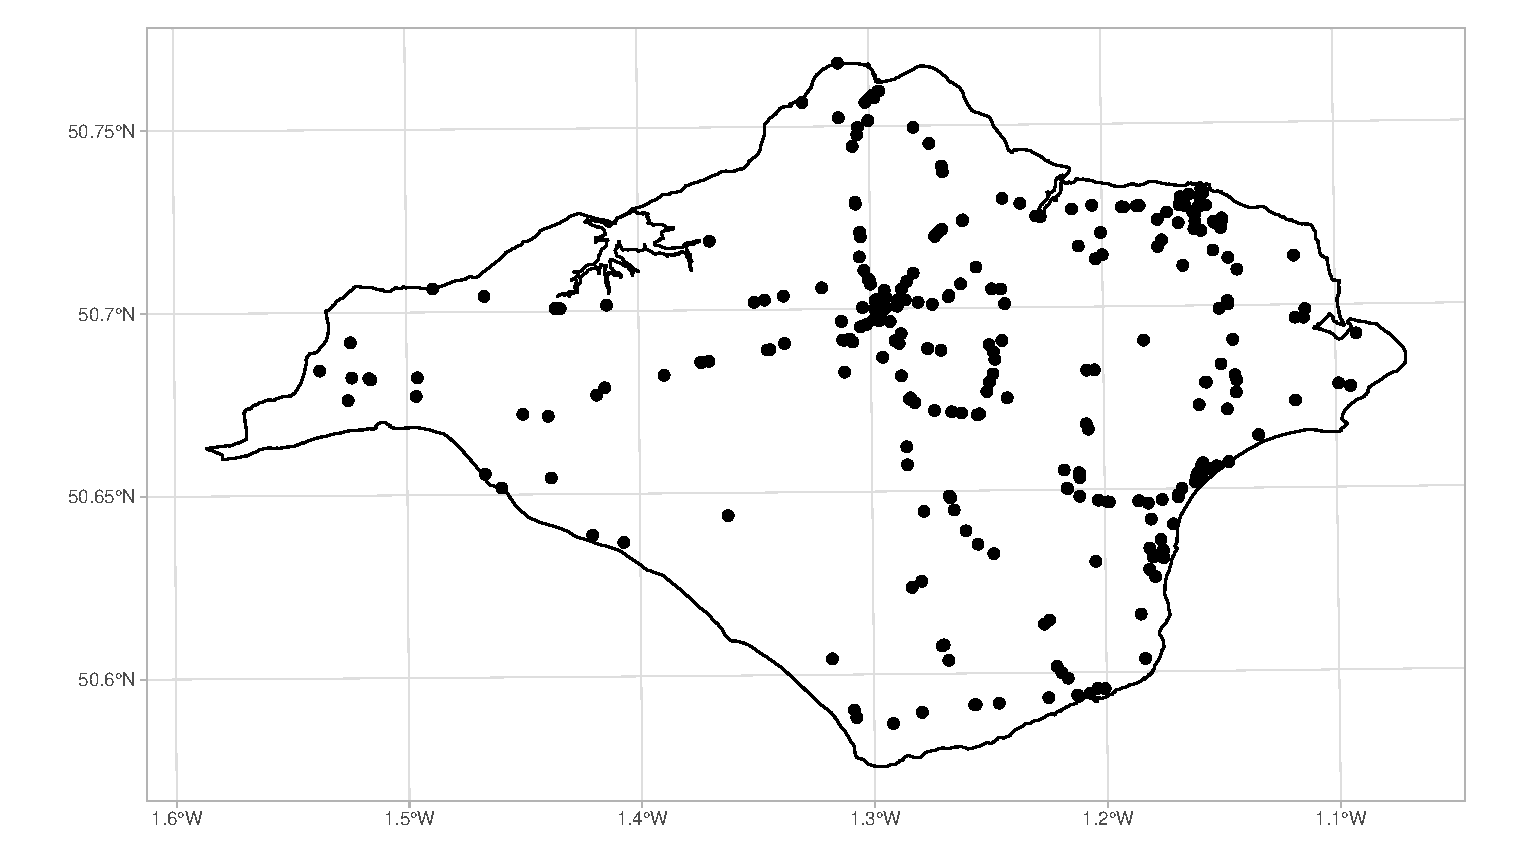
\includegraphics[width=\linewidth]{images/iow_crashes}
\end{figure}
\end{frame}

\begin{frame}
\frametitle{Point Processes on a Street Network}
\vspace{-0.25cm}
Car crashes represent a classical example of a point process occurring on a linear network and the usual statistical techniques (as the following quadratcount) are not valid. 
\vspace{-0.5cm}
\begin{figure}
	\centering
	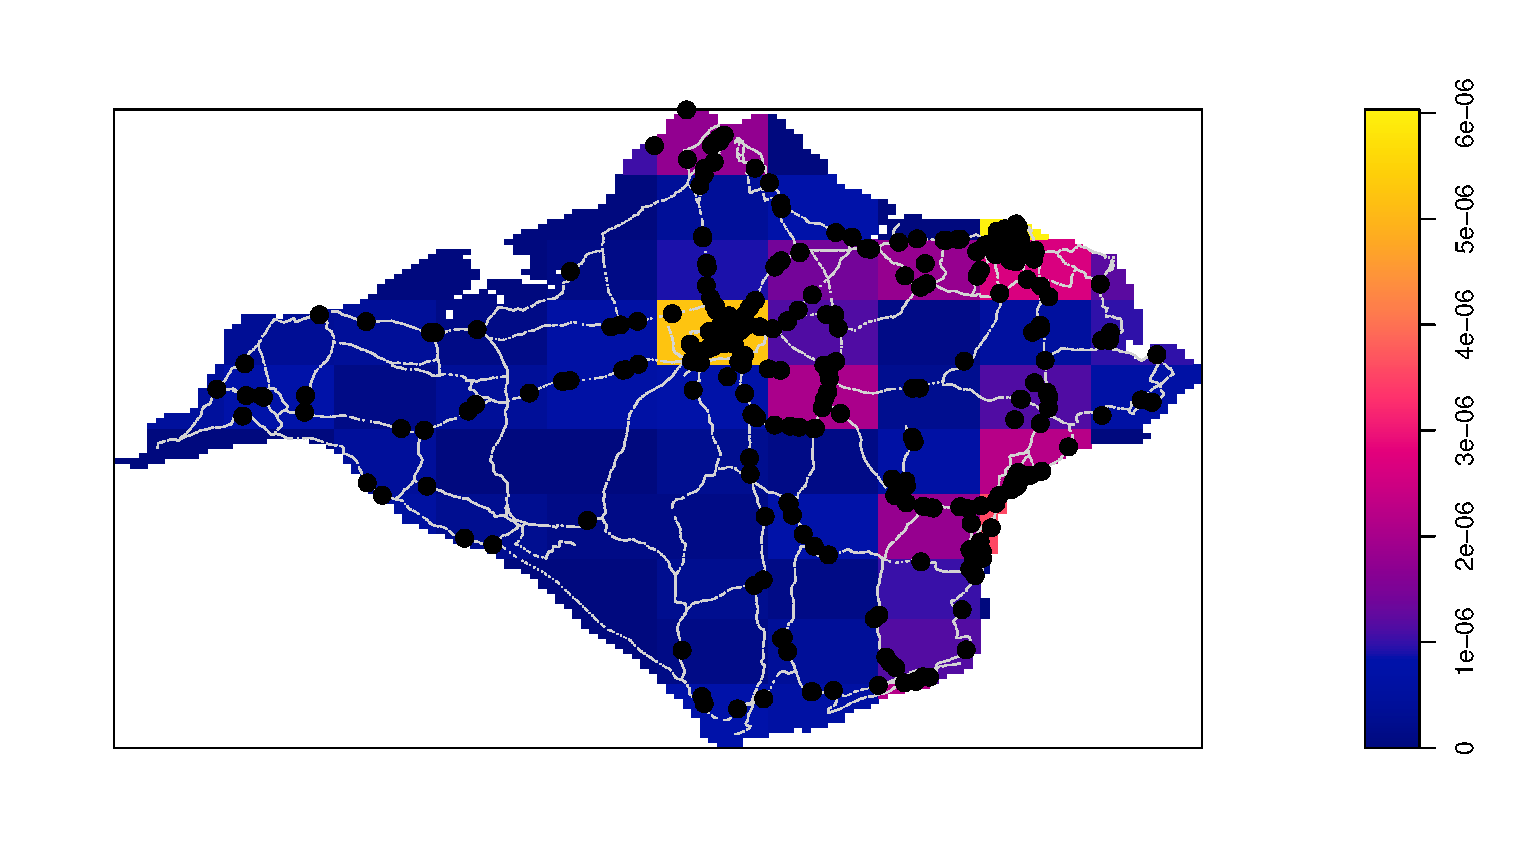
\includegraphics[width=\linewidth]{images/quadratcount2}
\end{figure}
\end{frame}

\begin{frame}
\frametitle{Street Networks}
\vspace{-0.75cm}
\begin{itemize}
  \setlength\itemsep{1em}
  \item The road network we use is built using OpenStreetMap data. 
  \item OpenStreetMap is a project that aims at building a free and editable map of the World with an open-content license. 
  \item The basic components of OpenStreetMap data are called \textit{elements} and they consist of: 
  \begin{itemize}
    \setlength\itemsep{0.25em}
    \item \textit{nodes}: representing points on the earth surface; 
    \item \textit{ways}: which is an ordered list of nodes; 
    \item \textit{relations}: which is a list of nodes, ways and other relations. Each member has additional information that describe its relationship with the other elements. Roads, turn restrictions and administrative boundaries are usually described as relations.
  \end{itemize}
\end{itemize}
\end{frame}

\begin{frame}
\frametitle{Street Network in the Isle of Wight}
This is a graphical representation of the main roads in the Isle of Wight. 
\vspace{-0.75cm}
\begin{figure}
\centering
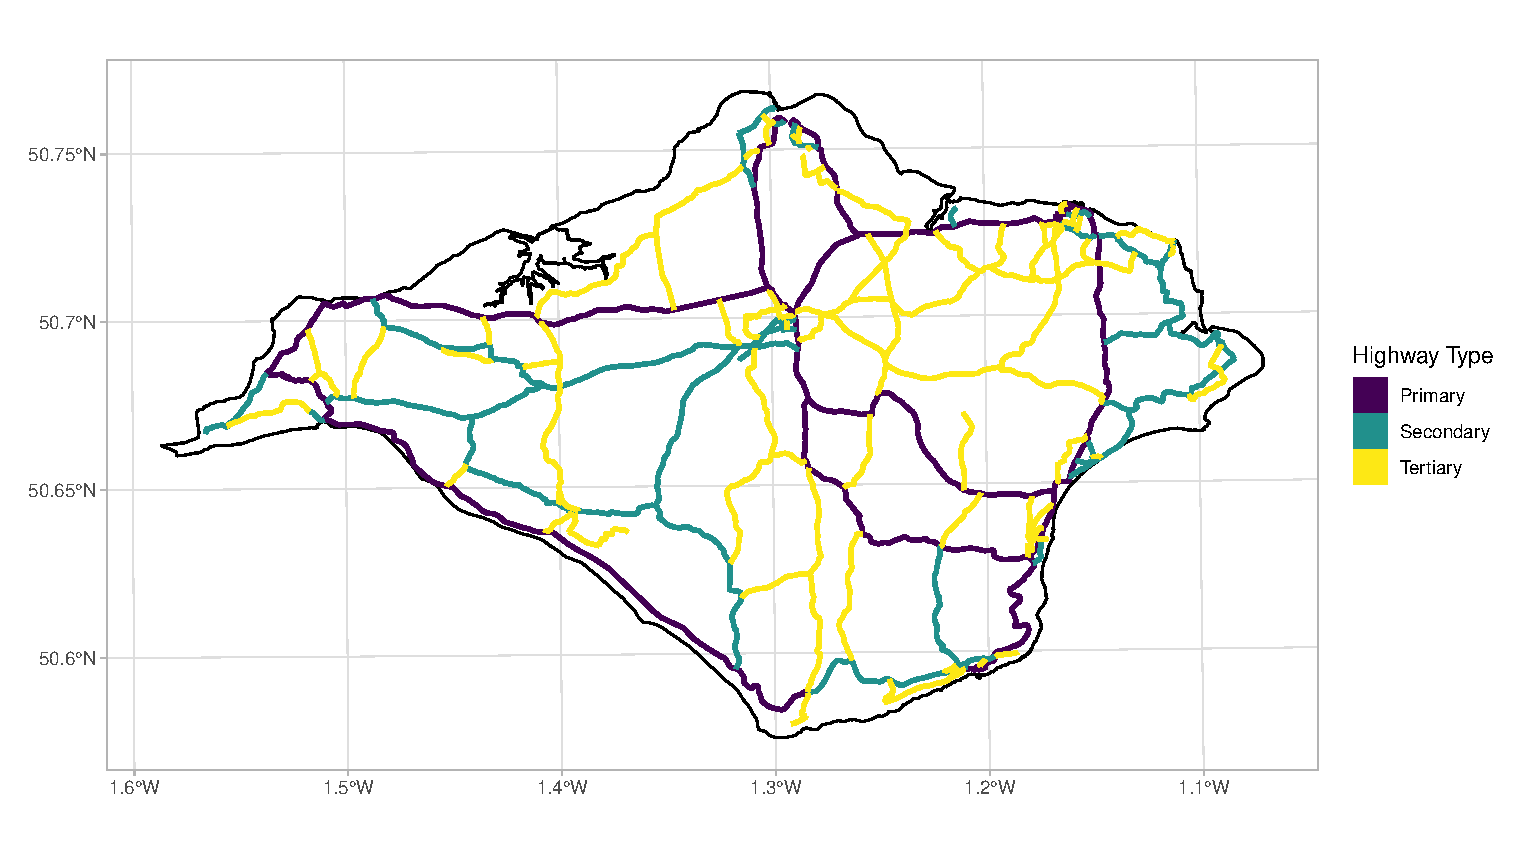
\includegraphics[width = 1.05\linewidth]{images/highway_type}
\end{figure}
\end{frame}

\begin{frame}
  \frametitle{\texttt{stplanr} - networks}
  \vspace{-0.75cm}
  \begin{itemize}
    \setlength\itemsep{1em}
    \item Broadly speaking, let's say that a street network is a network whose nodes and edges are associated with geographical elements in the space. 
    \item In the \texttt{stplanr} representation of a street network, the edges are the ways that were download from OSM while the vertexes are the starting and ending node of each way. 
    \item This representation implies that two or more edges are \textit{connected} if and only if they share one or more boundary point. 
  \end{itemize}
\end{frame}

\begin{frame}
  \frametitle{Problems...}
  \vspace{-0.5cm}
  Theories and definitions are fine but obviously the data we face in the wild world is quite different. We will discuss three probems: \textbf{roundabouts} (i.e. circular ways), \textbf{overpasses} (i.e. intersecting ways that are not really connected due to a vertical grade of separation) and (some) \textbf{street intersections}.  
  \begin{columns}
  	\begin{column}{0.5\linewidth}
  		\begin{figure}
  			\centering
  			\Large \textbf{Theory} \par \medskip
  			\includegraphics[width = \linewidth]{images/theory.png}
  		\end{figure}
  	\end{column}
  	\begin{column}{0.5\linewidth}
  		\begin{figure}
  			\centering
  			\Large \textbf{Real Data} \par \medskip
  			\includegraphics[width = \linewidth]{images/real_data.png}
  		\end{figure}
  	\end{column}
  \end{columns}
\end{frame}

\begin{frame}
  \frametitle{Roundabouts, i.e. circular ways}
  \vspace{-0.25cm}
  The roundabout on the left is unroutable by \texttt{stplanr}-definition of spatial network since the roundabout is not connected to the other edges.  
  \vspace{-0.55cm}
  \begin{columns}
    \begin{column}{0.5\linewidth}
      \begin{figure}
      \centering
      \large \textbf{Before} \par \medskip
      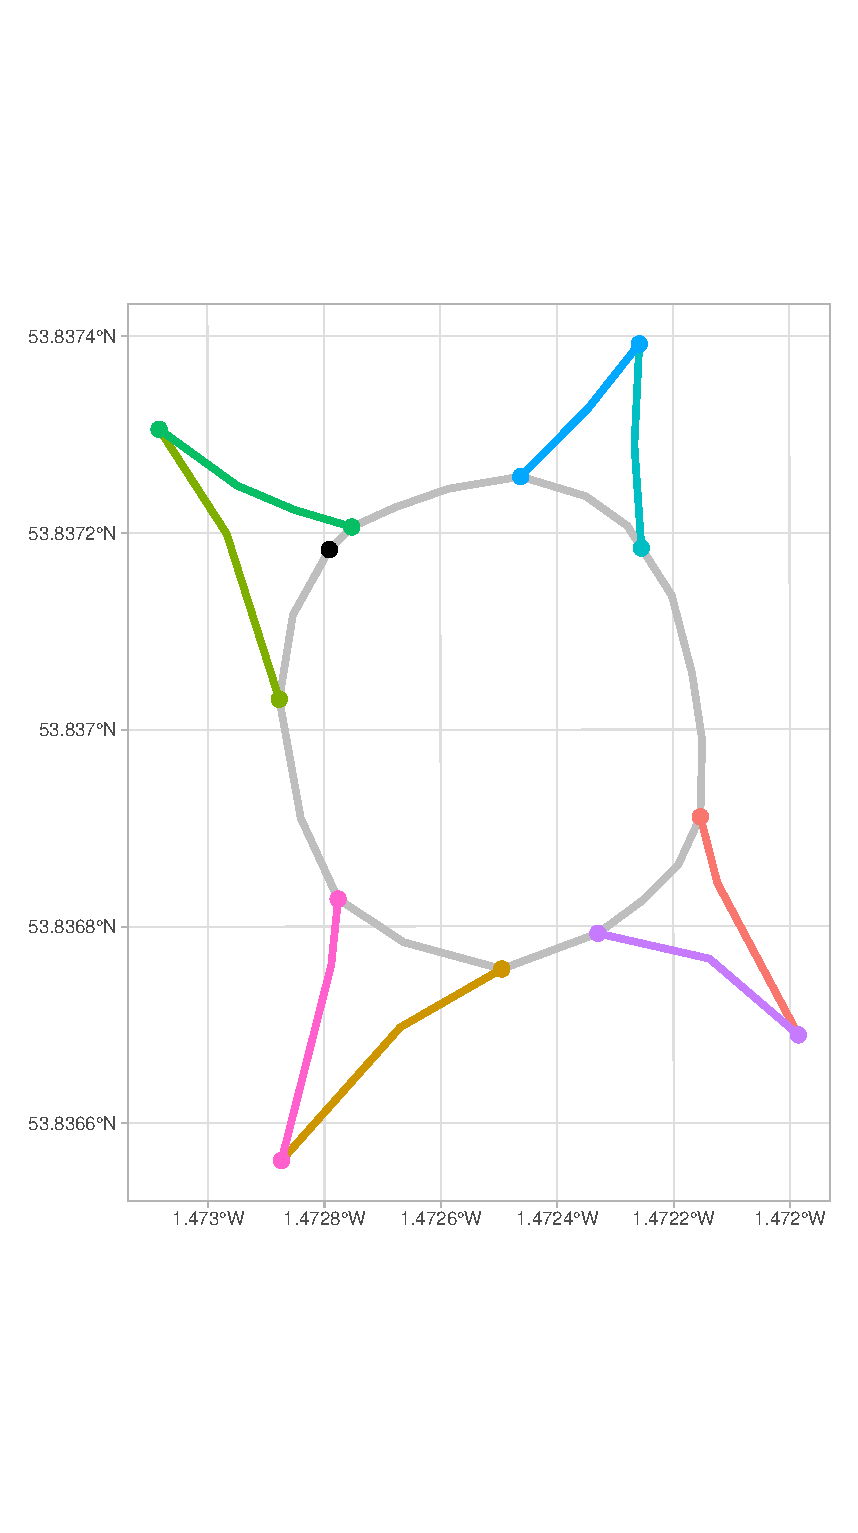
\includegraphics[width = 0.9\linewidth, trim = {0 0 0 4cm}, clip]{images/roundabout1}
      \end{figure}
    \end{column}
    \begin{column}{0.5\linewidth}
      \begin{figure}
      \centering
      \large \textbf{After} \par \medskip
      \includegraphics[width = 0.9\linewidth, trim = {0 0 0 4cm}, clip]{images/roundabout2}
      \end{figure}
    \end{column}
  \end{columns}
\end{frame}

\begin{frame}
\frametitle{Bridges, overpasses and underpasses}
\vspace{-0.75cm}
Even if we break up a street network (unroutable on the left) we must be sure  not to ruin overpasses and underpasses relations. 
\begin{columns}
	\begin{column}{0.5\linewidth}
		\begin{figure}
			\centering
			\large \textbf{Before} \par \medskip
			\includegraphics[width = \linewidth, trim = {4cm 0 3.75cm 0}, clip]{images/overpasses1}
		\end{figure}
	\end{column}
\begin{column}{0.5\linewidth}
	\begin{figure}
		\centering
		\large \textbf{After} \par \medskip
		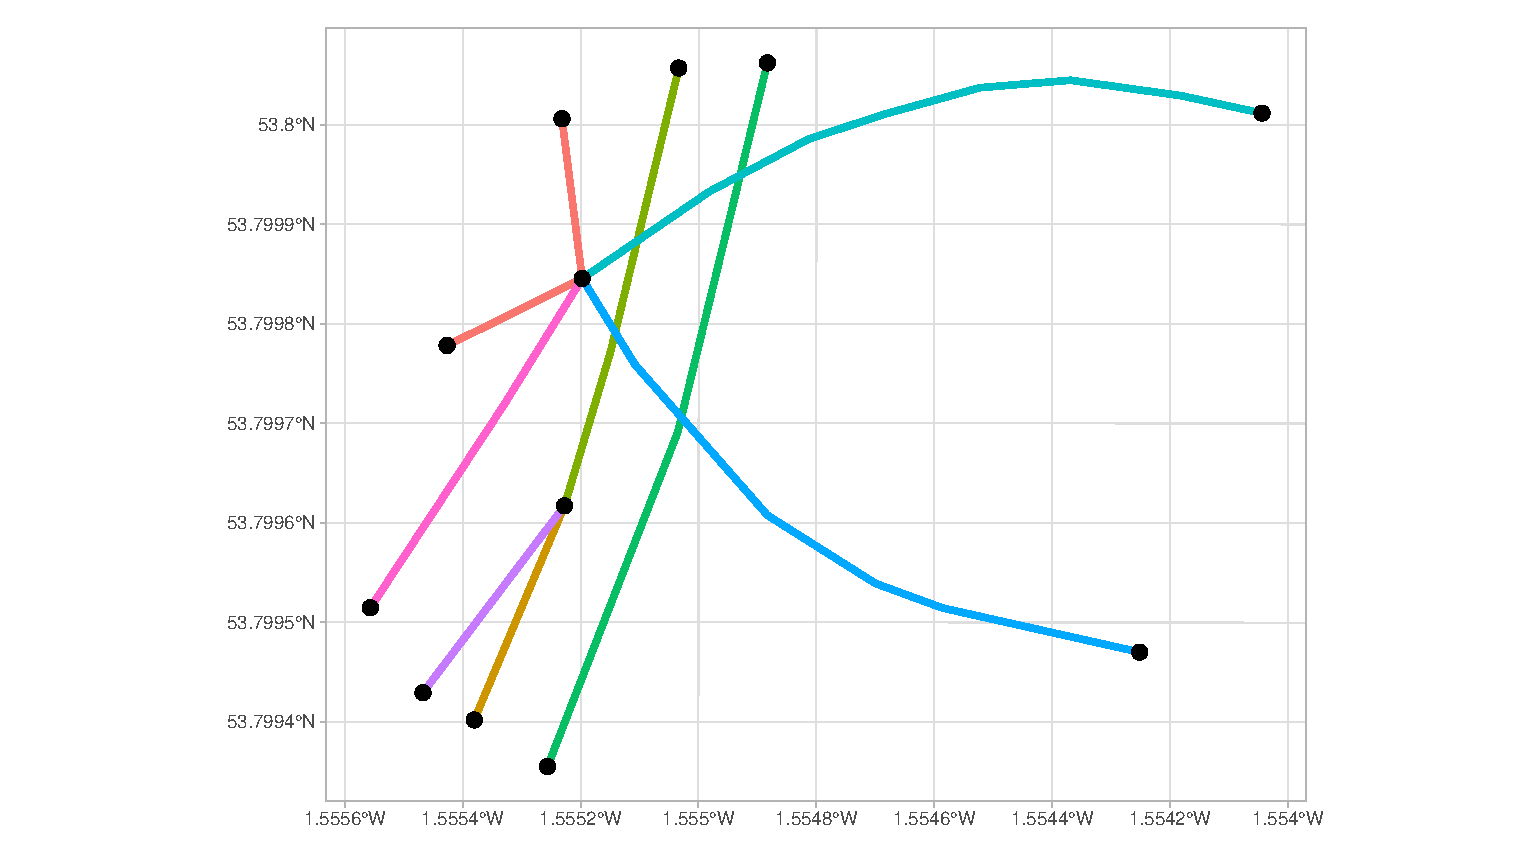
\includegraphics[width = \linewidth, trim = {4cm 0 3.75cm 0}, clip]{images/overpasses2}
	\end{figure}
\end{column}
\end{columns}
\end{frame}

\begin{frame}
\frametitle{Streets intersections}
\vspace{-0.75cm}
There are also some cases where two streets intersects and they don't share any vertex.
\begin{columns}
	\begin{column}{0.5\linewidth}
		\begin{figure}
			\centering
			\large \textbf{Before} \par \medskip
			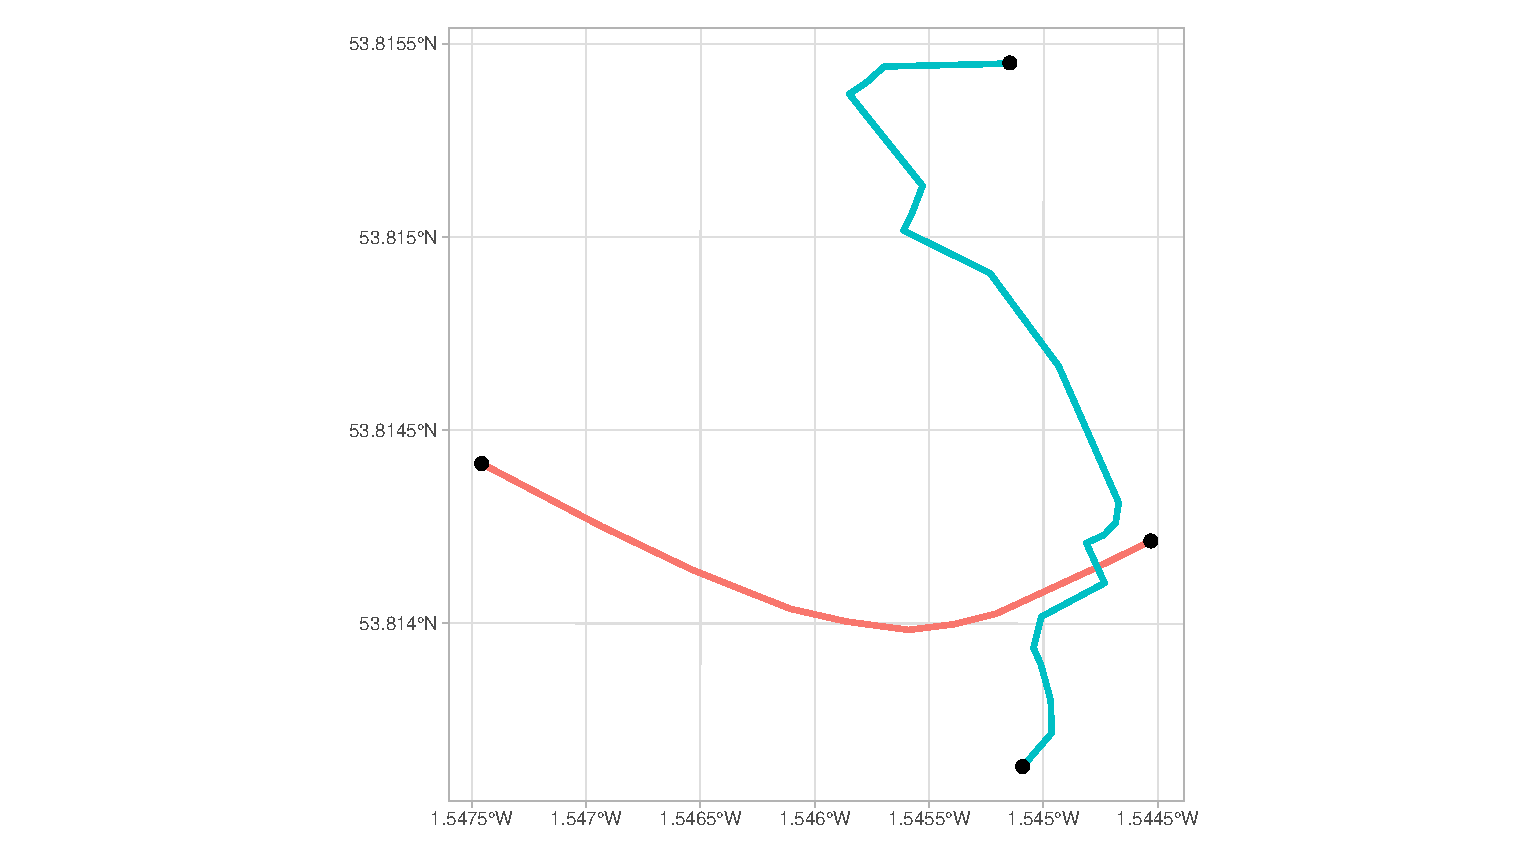
\includegraphics[width = \linewidth, trim = {5.5cm 0 4.5cm 0}, clip]{images/intersections1}
		\end{figure}
	\end{column}
\begin{column}{0.5\linewidth}
	\begin{figure}
		\centering
		\large \textbf{After} \par \medskip
		\includegraphics[width = \linewidth, trim = {5.5cm 0 4.5cm 0}, clip]{images/intersections2}
	\end{figure}
\end{column}
\end{columns}
\end{frame}

\begin{frame}
\frametitle{Fixing the street networks}
\vspace{-0.25cm}
We developed a new function (called \texttt{rnet\_breakup\_vertices} and stored in \texttt{stplanr} package) to fix all these problems and this is the result. 
\begin{figure}
	\centering
	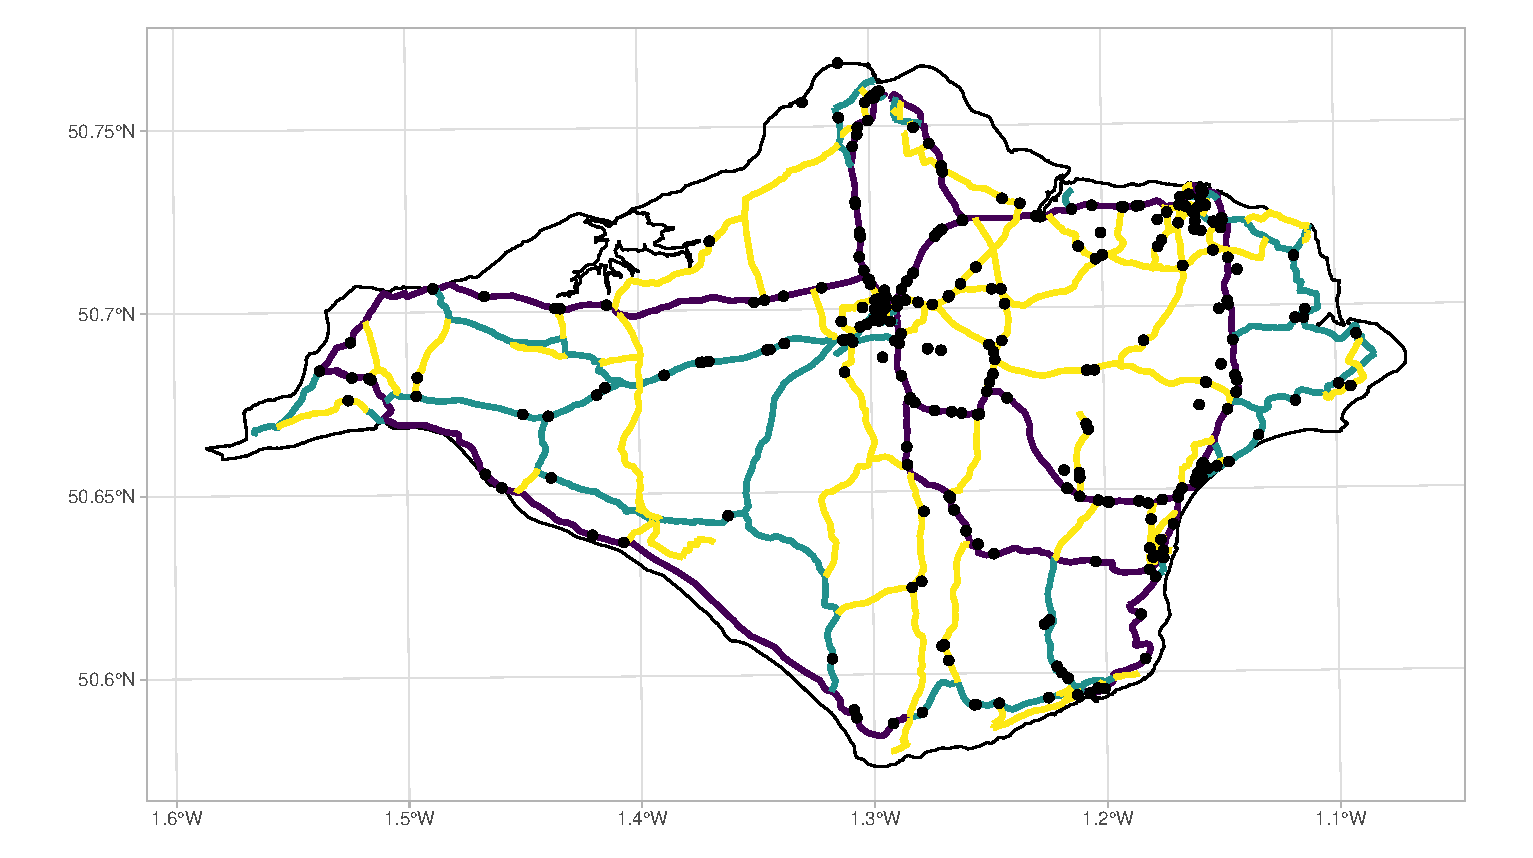
\includegraphics[width=\linewidth]{images/breaking_network}
\end{figure}
\end{frame}

\begin{frame}
\frametitle{Modeling of crashes on street networks}
Summary of the models
\end{frame}

\begin{frame}
\frametitle{Counting crashes on street networks}
\vspace{-0.75cm}
\begin{itemize}
	\setlength\itemsep{1em}
	\item Following the same ideas behind the quadratcounts on the plane (and some statistical theories) we wrote a few function to count the number of car crashes occurring on each edge of the street network. 
	\item R can only represent exactly integers numbers and fractions whose denominator is a power of two (source), so none of the car crashes (whose coordinates are represented as double numbers with a 53 binary digits accuracy) lie exactly on the street network.
	\item For that reason we wrote a few R function to match each car crash with the nearest edge on the network and count the occurrences.
\end{itemize}
\end{frame}

\begin{frame}{The first road risk measure}
\vspace{-0.25cm}
This is the result. You should note that we excluded all car crashes that were farther than 100m from the nearest network edge (33  crashes). 
\begin{figure}
	\centering
	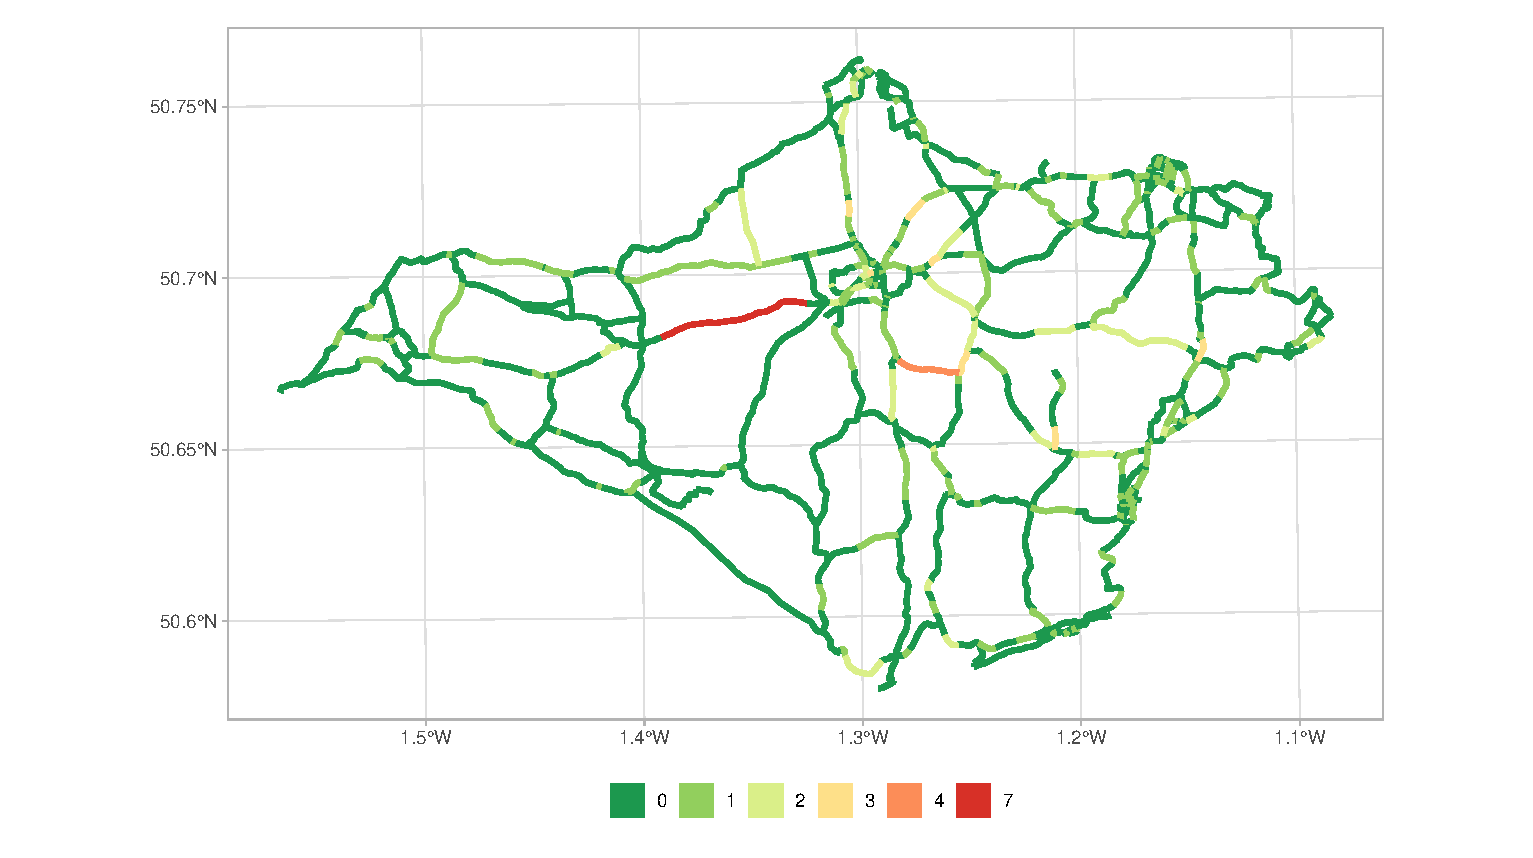
\includegraphics[width=\linewidth]{images/count_on_nearest_street}
\end{figure}
\end{frame}

\begin{frame}{The first road risk measure}
\vspace{-0.25cm}
This is the result. You should note that we excluded all car crashes that were farther than 100m from the nearest network edge (33  crashes). 
\begin{figure}
	\centering
	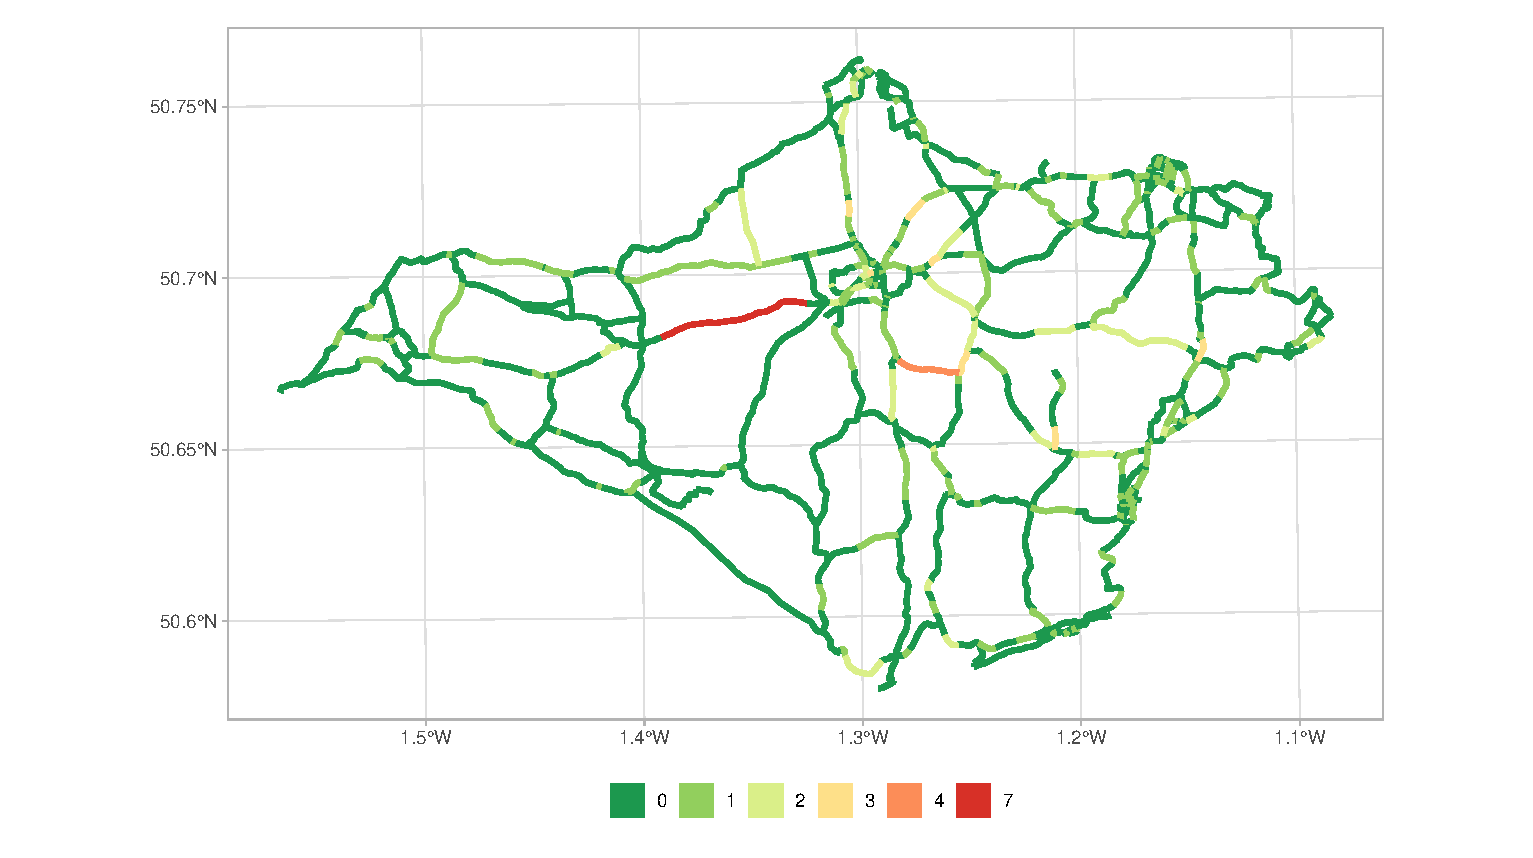
\includegraphics[width=\linewidth]{images/count_on_nearest_street}
\end{figure}
\end{frame}

\begin{frame}{Problems with the raw counts measure}
\begin{itemize}
	\setlength\itemsep{1em}
	\item There are some clear problems with the previous risk measure and, the most important one, is that we are comparing ways with very different length (which is what we are going to call \textit{exposure}). 
	\item There are two possible solutions: 1) rebuild the network cutting and pasting ways in such a way that they all have approximately the same length; 2) estimate the number of car crashes per meter. 
	\item For the moment we are working with the second solution since the other one is much more difficult to implement. 
\end{itemize}
\end{frame}

\begin{frame}{Car crashes per meter}
\vspace{-0.25cm}
This is the result and, then again, there are some obvious problems: there are a few car crashes occurring in very small road segments that artificially inflate this risk index.  
\begin{figure}
	\centering
	\includegraphics[width=\linewidth]{images/car_crashes_per_meter}
\end{figure}
\end{frame}

\begin{frame}{Smoothing on a linear network}
\begin{itemize}
	\setlength\itemsep{1em}
	\item Let $n$ be the number of edges in the street network, $x_i, \ i = 1,\dots,n$ the number of car crashes occurring in each edge and $m_i, \ i = 1\dots n$ the length of each way. 
\end{itemize}
\end{frame}

\begin{frame}{Smoothing on a linear network}
\vspace{-0.25cm}
This is the result with = 6. We'll talk later on how to choose that value. Now it's possible to extract some information from that plot. 
\begin{figure}
	\centering
	\includegraphics[width=\linewidth]{images/car_crashes_per_meter_smooth6}
\end{figure}
\end{frame}

\begin{frame}{Why network cleaning is important?}
\begin{itemize}
	\setlength\itemsep{1em}
	\item To solved that new problem
\end{itemize}
\end{frame}

\begin{frame}
\frametitle{TODO}
\begin{itemize}
	\item Add citations and fix bibliography
	\item Add credits to memes, OSM and beamer theme
	\item highlight important word (i.e. \alert{ABC})
\end{itemize}
\end{frame}
\end{document}
